% !TEX encoding = UTF-8 Unicode

\chapter{La \mt d'analyse ondelette}
\label{chap4}

\section {Méthodologie}
Dans le domaine traitement du signal, la transformée de Fourier (FT) est un outil mathématique important car elle est un pont de connexion très important pour la représentation du signal entre le domaine spatial et le domaine fréquentiel. La transformée de Fourier est appelée la représentation du domaine de fréquence du signal origine. Le terme transformée de Fourier fait référence à la fois à la représentation dans le domaine fréquentiel et à l'opération mathématique qui associe la représentation du domaine fréquentiel à une fonction du temps. La figure \ref{Pic4_1} montre une exemple sur la représentation les signals de la taux d'infection et le température moyenne du province Cantho - Vietnam et leurs transformée de Fourier. 

\begin{figure}[h]
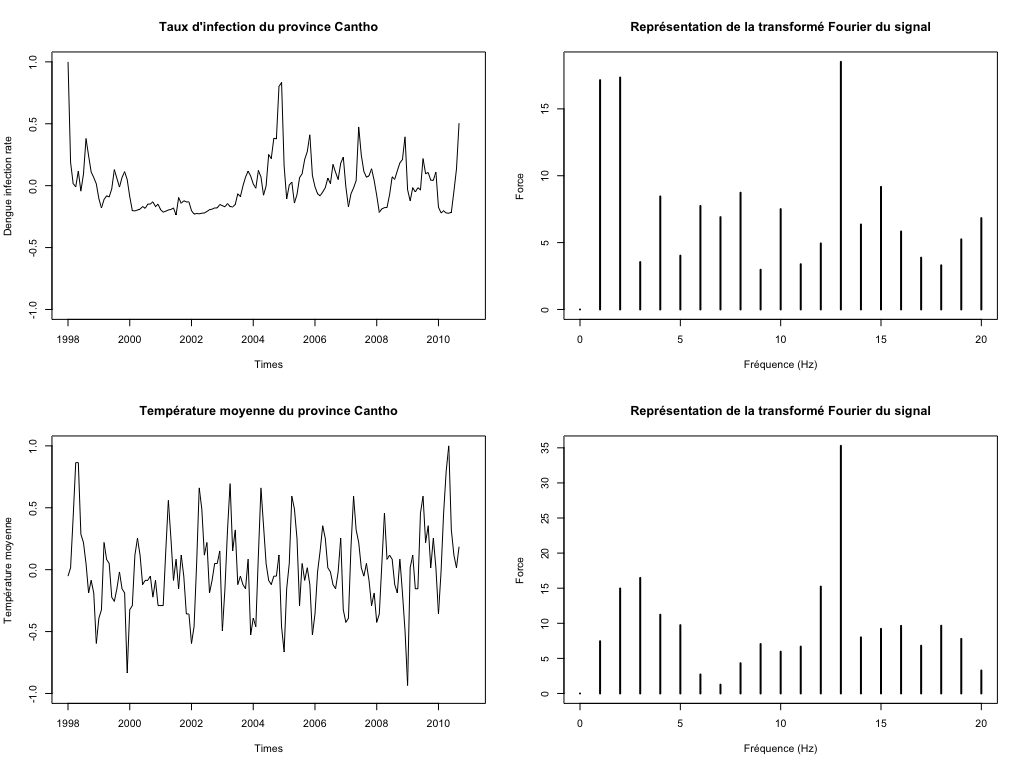
\includegraphics[width = \linewidth]{../figures/chap4/Pic4_1.png}
\caption{Exemple de la transformée de Fourier}
\label{Pic4_1}	
\end{figure}

On peut trouve que les spectre de Fourier montre les composantes de fréquence du signale mais n'indique pas où les fréquences apparaissent. La transformée de Fourier fournit uniquement des information globales et ne convient qu'aux signaux circulaire. Elle n'est pas contenu des mutation ou de changement imprévisibles. Pour surmonter cette défaut, Gabor \cite{gabor1946} a appliqué la transformée de Fourier (Windowed Fourier Transform - WFT ) par fenêtre à chaque petit segment du signal. Pour surmonter cet inconvénient, Gabor a appliqué la transformée de Fourier de la fenêtre à chaque petit segment du signal (fenêtre); Cette transformation montre la relation entre l'espace et la fréquence mais est régie par le principe d'incertitude de Heisengber pour les composantes à haute fréquence et à basse fréquence dans le signal \cite{kaiser1994}. En 1975, Zweig a développé une méthode de multirésolution, qui utilise une impulsion oscillante pour redimensionner et comparer des signaux dans les segments individuels. Cette impulsion est appelée une "ondelette" (qui traduit à partir de son origine une petite onde). Cette technique utilise une ondelette contenant des oscillations de basse fréquence et le compare avec le signal analytique pour trouver des information globale du signal dans la résolution brute. Ensuite, on compresse les petites ondes (cette étape est appelé mise à échelle) pour augmenter progressivement la fréquence d'oscillation. Dans les étapes suivant, le signal sera étudié en détail à des résolution plus élevées pour détecter les composants rapides qui reste cachés dans le signal.

La transformée en ondelette est plus flexible par rapport à la transformée de Fourier car il n'est pas nécessaire d'utiliser une fonction d'ondelette fixe et il peut sélectionner les différentes fonctions d'ondelettes pour être adapté au problème qui convient. Les ondelettes qui constituent une famille de fonction dérivée d'une seule fonction qui s'appelle "ondelette mère" dénoté par $\Psi_{\alpha, \,\tau} (t)$. Cette "ondelette mère" a été exprimé sous forme une fonction avec deux paramètre, l'un est le paramètre qui exprimer la position du temps $\tau$, l'autre est l'échelle de l'ondelette $\alpha$, qui corresponde au fréquence. Plus précisement, l'ondelette est définit comme
$$\Psi_{\alpha, \tau} = \frac{1}{\sqrt{\alpha} }\Psi \left ( \frac{t - \tau}{\alpha} \right ) $$
Une des formes ondelette qu'on utilise très souvent est ondelette Morlet. L'ondelette Morlet est définie comme
$$  \Psi (t) = \pi^{-1/4} exp (- i2\pi f_0 t) exp \left ( \frac{-t^2}{2} \right ) $$
Une transforme d'ondelette d'une série temporelle x(t) avec une "ondelette mère" est performé comme 
$$  W_x(\alpha, \tau) =  \frac{1}{\sqrt{\alpha}} \, \int_{-\infty}^{\infty} x(t) \Psi^\ast \left (  \frac {t - \tau} {\alpha}    \right ) dt = \int_{-\infty}^{\infty} x(t)\Psi^{\ast}_{\alpha,\tau} (t) dt $$
où l'astérisque indique la forme conjugué complexe. Le coefficient d'ondelette $W_x(\alpha, \tau)$ représente le contribution de l'échelle $\alpha$ du signal donc le temp était dans une différente position $\tau$. Le calcul de la transformée en ondelette du signal x(t) se fait en augmentant le paramètre $\tau$ sur une rayon d'échelle $\alpha$ jusqu'à ce que toutes les structures cohérentes dans le signal peuvent être identifiés. 
Avec l'approche ondelette, on peut estimer la répartition de la variance entre l'échelle $\alpha$ et la différence emplacement du temps $\tau$. Il est connu comme le spectre de puissance ondelette : $S_x(f,\tau) = |W_x(f,\tau)|^2$. Pour quantifier les relations statistiques entre les deux séries temporelles, la cohérence des ondelette peut être calculer
$$ R_{x,y} (f,\tau) = \frac{|<W_{x,y}(f,\tau)>|^2}{|<W_{x}(f,\tau)>|^2| <W_{y}(f,\tau)>|^2}  $$
où les crochets autour des termes indiquent le lissage dans le temps et la fréquence, $W_{x}(f,\tau)$ est la transforme ondelette de la série x(t), $W_{y}(f,\tau)$ est la transforme ondelette de la série y(t) et $W_{x,y}(f,\tau) = W_{x}(f,\tau)*W_{y}(f,\tau)$ est la transforme de la coupe d'ondelette. La cohérence des ondelettes fournit des informations locales sur l'endroi où deux signaux non stationnaires, x(t) et y(t), sont linéaire corrélés à une fréquence particulière(ou période). $R_{x,y} (f,\tau)$ est égale à un quand il y aura une relation linéaire parfaite à un moment donné et la fréquence entre les deux signaux.

\section{Résultats d'expérimentaux}

Dans notre recherche, nous appliquons cette méthode pour analyser la relation entre les taux d'inflections et les variables environnementaux des 64 provinces du pays Vietnam dans la période Janvier 1998 au Septembre 2010. La raison pour laquelle nous choisissons le Vietnam et cette période est due à l'exhaustivité  et la continuité des données. Pour chaque province au Vietnam, nous calculons la latitude et la longitude moyenne et leurs comparé avec ceux des stations climatiques. Puis nous choisissons le station climatique le plus proche de cette province et le prendre leurs variables climatiques pour calculer la cohérence des ondelette avec le taux d'inflection de la province observé. La figure \ref{Pic4_2} montre la schéma d'application la méthode d'analyse ondelette sur les données du Vietnam. 

\begin{figure}[h]
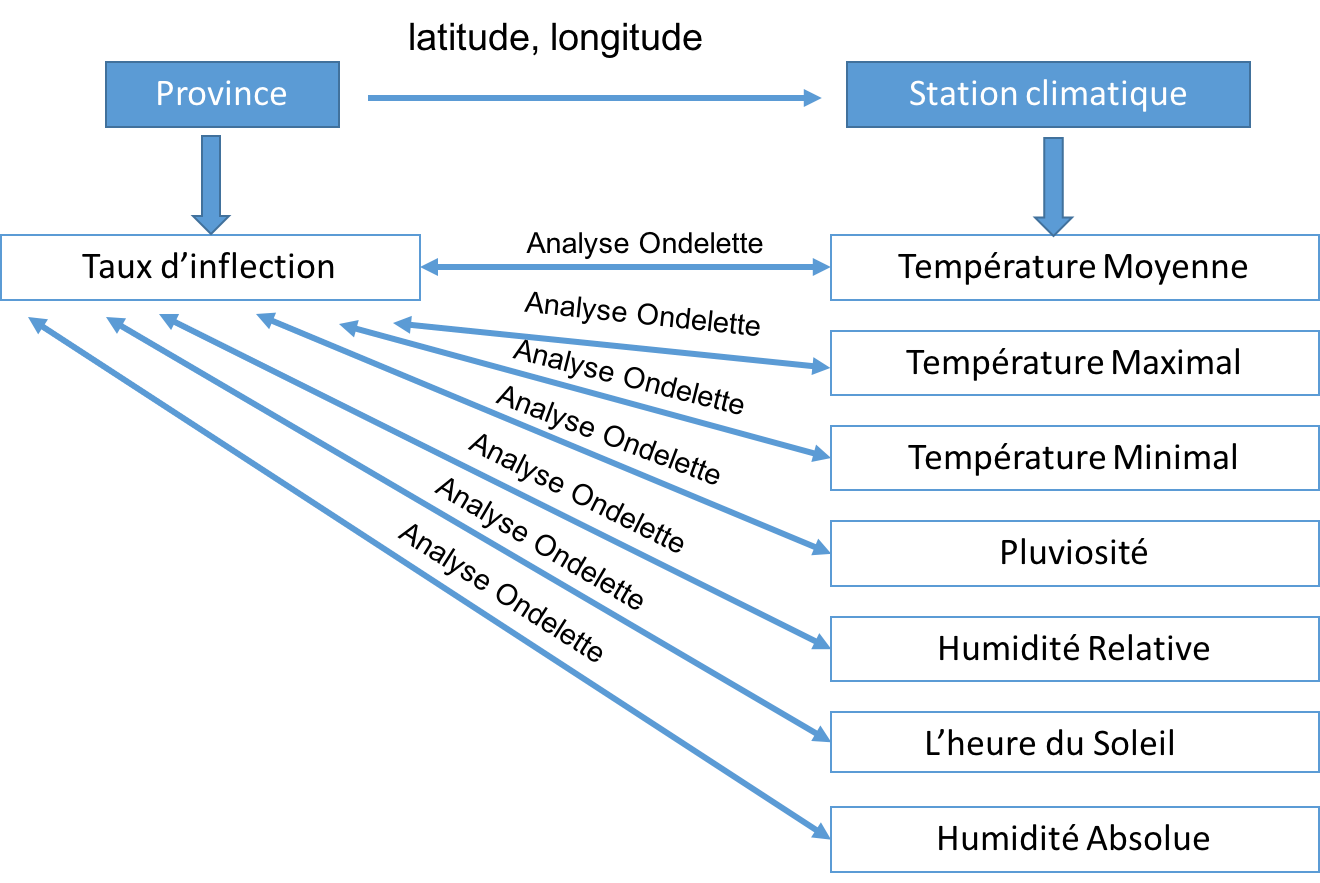
\includegraphics[width = \linewidth]{../figures/chap4/Pic4_2.png}
\caption{La processus d'appliquer la méthode analyse ondelette sur les données du Vietnam}
\label{Pic4_2}	
\end{figure}

Nous utilisont R version 3.3.1 sur RStudio version 1.1.442 pour calculer les résultats expérimentaux. La méthode d'analyse ondelette est définit dans le package "biwavelet" \cite{gouhier2018}. Nous choisissons les 3 typiques provinces : Hanoi, Da Nang et Ho Chi Minh qui travers les 3 régions du Vietnam pour montrer leurs résultats expérimentaux. 

La figure \ref{Pic4_3},\ref{Pic4_4}, \ref{Pic4_5} montre la résultat expérimental du province Hanoi et la relative humidité, Da Nang et l'heure du soleil, Ho Chi Minh et la température moyenne . Les figures \ref{Pic4_3} (a), \ref{Pic4_4} (a), \ref{Pic4_5} (a) montrent les deux signaux qui ont été normalisé. Le signal de la dengue est en couleur rouge et les facteurs climatiques est en couleur bleu. La figure  \ref{Pic4_3} (b), \ref{Pic4_4} (b), \ref{Pic4_5} (b) montrent la cohérence les deux signaux observé. Les régions en couleurs rouges sont les régions significant relative entre les deux signaux. Les flèches avec le direction à gauche qui indiquent les deux signaux sont en phase l'inverse, à droite qui indiquent les deux signaux sont en phase. Les flèches pointant vers le haut signifient que le taux d'inflection de la dengue conduit le facteur climatique par $\pi/2$ et s'ils pointant vers le bas signifient que le facteur climatique conduit le taux d'inflection par $\pi/2$. 

On peut facilement détecter des grandes corrélations entre Hanoi et l'humidité relative. Pendant la période 1998 - 2003 et 2005 - 2010, la taux d'inflection à Hanoi et l'humidité relative sont toujours en phase l'inverse dans la période 2 mois. Ceci est dû au fait que le climat du nord du Vietnam est relativement élevé et humide toute l'année, et que le climat est fortement influencé par la Chine continentale et qu'il a un climat continental.  

Dans le cas de Da Nang, une  grande province au Centre du Vietnam avec le climat tropical mousson, on trouve une  serré relation entre l'épidémie de la dengue à Da Nang avec l'heures de soleil.  Ici le climat de Da Nang avait la transition entre le climat xavan du Sud et le climat subtropical du Nord du Vietnam. Puis, il existe aussi la mousson du Sud-ouest qui souffle du golfe de Thaïlande et au-dessus des montagnes de Truong Son, il fera un temps chaud et sec pour toute la région. Entre 2003 - 2010, les deux signaux sont corrélé aux période 1 mois et l'heure du soleil conduit la taux d'infection par $\pi/2$. Tandis que  1998 - 2010 ils sont totalement corrélé en phase  aux période 4 mois. 

Le troisième cas est Ho Chi Minh ville, qui est considérée comme la capital du Sud-Vietnam, qui appartient dans le région le climat tropical xavan avec des fortes précipitations et des températures élevées tout au long de l'année. C'est la raison pour laquelle on peut détecter une grande corrélation entre l'épidémie de la dengue et la température moyenne dans cette provinces. Les deux signaux montrent une association dans entre 1998 - 2000 et 2003 - 2010 sur la période 1 mois. La température moyenne a totalement conduit le taux d'infection par  $\pi/2$ dans ces deux temps.



\begin{figure}[h]
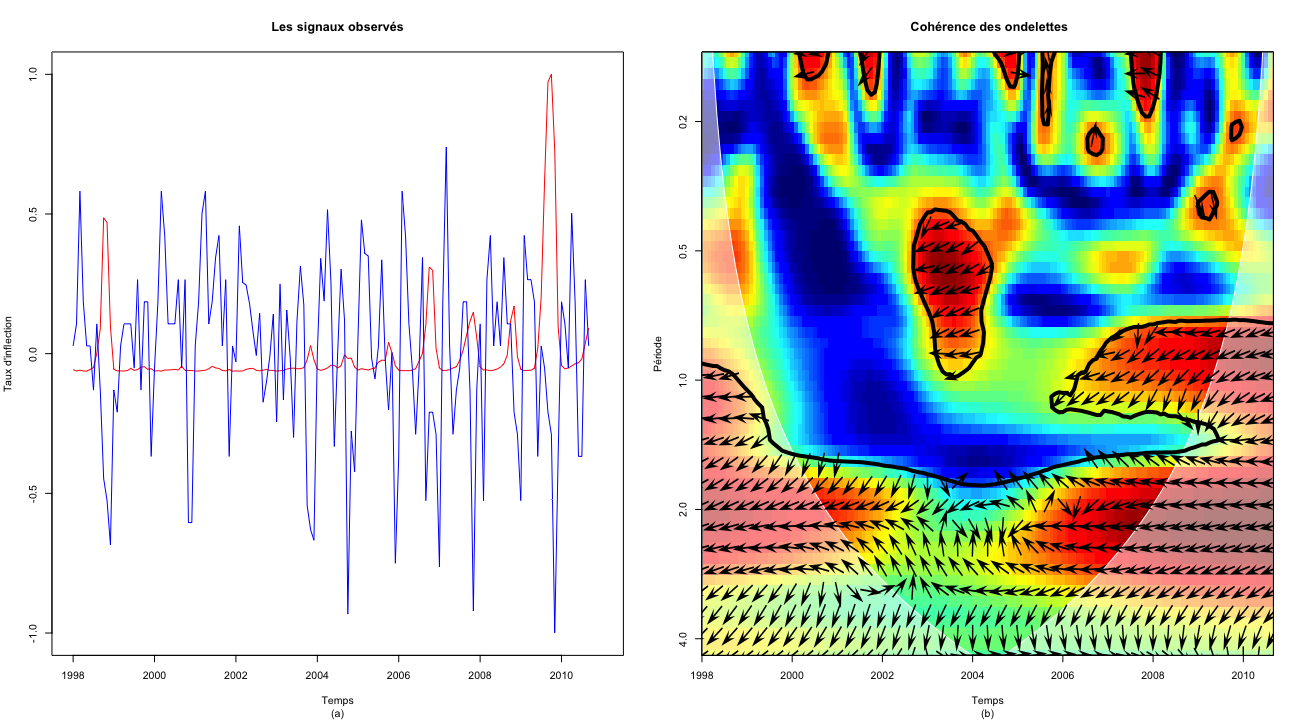
\includegraphics[width = \linewidth]{../figures/chap4/Pic4_3.png}
\caption{Cohérence des ondelettes entre le taux d'inflection de Hanoi et l'humidité relative. 
(a) Les signaux observé : le taux d'inflection est représenté en couleur rouge et l'humidité relative est représenté en couleur bleu.
(b) Cohérence des ondelettes entre le taux d'inflection de la dengue et l'humidité relative de Hanoi, calculée à l'aide de la fonction d'ondelette de Morlet. Les couleurs codent les valeurs de puissance du bleu foncé pour une faible cohérence au rouge foncé pour une cohérence élevée. Les lignes noir imbriquées montrent les niveaux de signification $\alpha$ = 5\% calculés sur la base de 1 000 séries amorcées. Le cône d'influence indique la région non influencée par les effets de bord. }
\label{Pic4_3}	
\end{figure}

\begin{figure}[h]
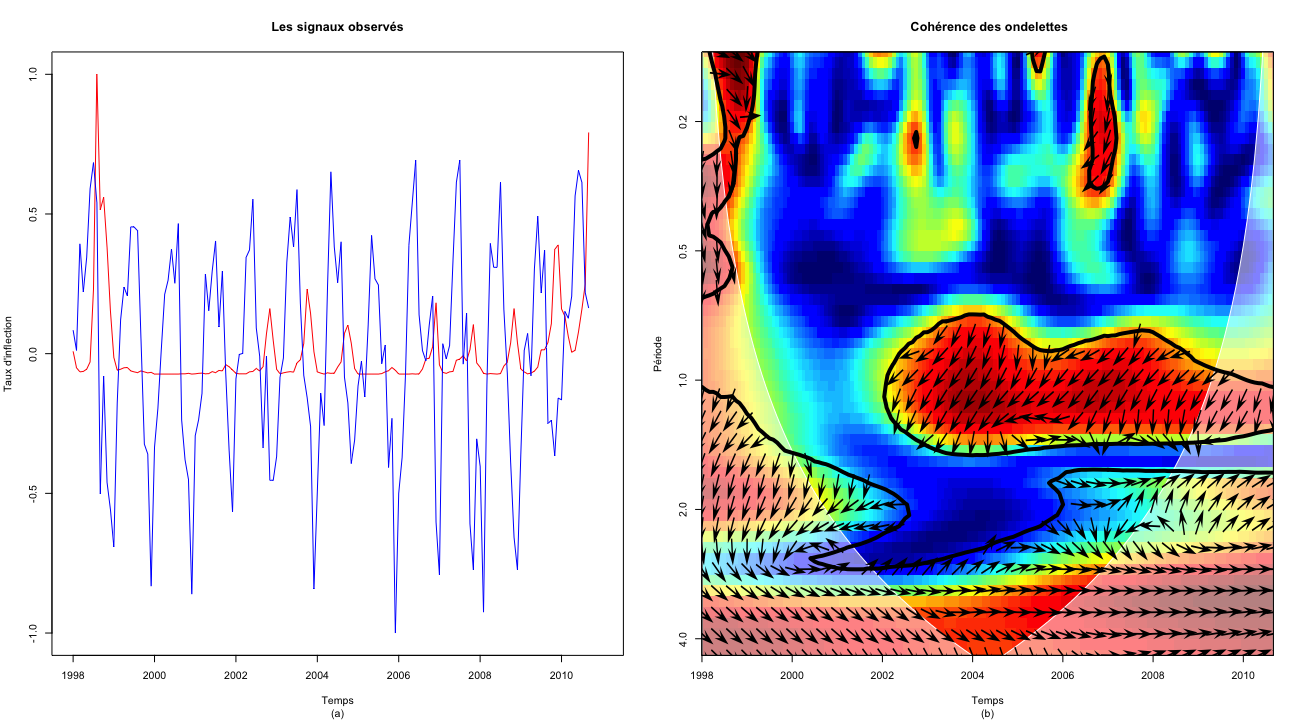
\includegraphics[width = \linewidth]{../figures/chap4/Pic4_4.png}
\caption{Cohérence des ondelettes entre le taux d'inflection de Da Nang et l'heure du soleil. 
(a) Les signaux observé : le taux d'inflection est représenté en couleur rouge et l'heure du soleil est représenté en couleur bleu.
(b) Cohérence des ondelettes entre le taux d'inflection de la dengue et l'heure du soleil de Da Nang, calculée à l'aide de la fonction d'ondelette de Morlet. Les couleurs codent les valeurs de puissance du bleu foncé pour une faible cohérence au rouge foncé pour une cohérence élevée. Les lignes noir imbriquées montrent les niveaux de signification $\alpha$ = 5\% calculés sur la base de 1 000 séries amorcées. Le cône d'influence indique la région non influencée par les effets de bord. }
\label{Pic4_4}	
\end{figure}

\begin{figure}[h]
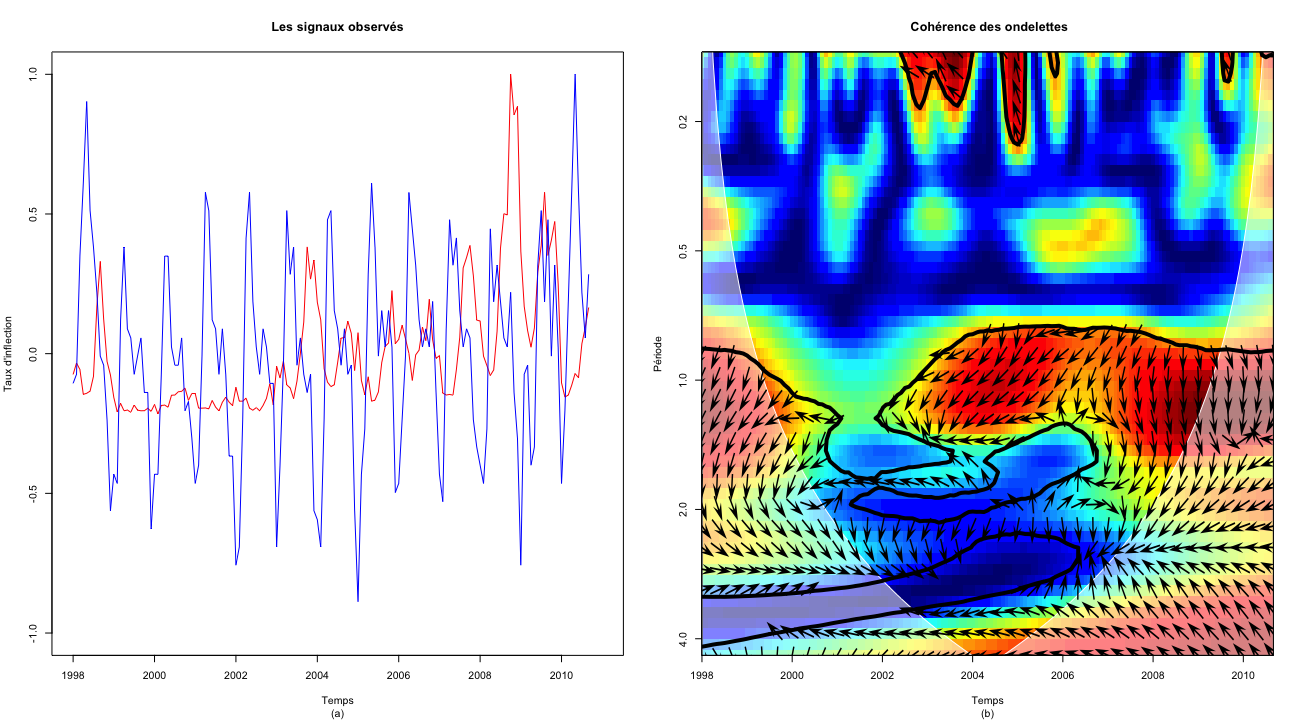
\includegraphics[width = \linewidth]{../figures/chap4/Pic4_5.png}
\caption{Cohérence des ondelettes entre le taux d'inflection de Ho Chi Minh ville et la température moyenne. 
(a) Les signaux observé : le taux d'inflection est représenté en couleur rouge et la température moyenne est représenté en couleur bleu.
(b) Cohérence des ondelettes entre le taux d'inflection de la dengue et la température moyenne de Ho Chi Minh ville, calculée à l'aide de la fonction d'ondelette de Morlet. Les couleurs codent les valeurs de puissance du bleu foncé pour une faible cohérence au rouge foncé pour une cohérence élevée. Les lignes noir imbriquées montrent les niveaux de signification $\alpha$ = 5\% calculés sur la base de 1 000 séries amorcées. Le cône d'influence indique la région non influencée par les effets de bord.}
\label{Pic4_5}	
\end{figure}

Les trois résultats ci-dessus montrent une serré relation entre les facteur climatiques les le situation d'infection de la dengue dans des trois grandes provinces du Vietnam. Nous allons ensuite procéder une analyse complète des liens entre les 7 facteurs climatiques et la situation épidémique de la dengue sur 64 provinces du Vietnam pour avoir une point vue global de l'influence des facteurs climatiques sur l'épidémie de la dengue. Pour chaque provinces au Vietnam, on applique la méthode d'analyse ondelette pour calculer la cohérence entre la taux d'infection de cette province avec chaque facteurs climatique. Puis, on calcule 
le taux significatif en divisant la somme des régions significatifs par l'ensemble des cohérences des 2 signaux. On définit 
$$\tau = \frac{R}{C}$$

où $R$ est la somme total des région significatif parmi des cohérence des 2 signaux et $C$ est le nombre total des cohérences des 2 signaux. On conclus que la relation entre la situation de la dengue et le facteur climatique d'une province est significatif si son taux significatif est supérieur au seuil $s$ : 
$$\tau \geq s, 0 < s < 1$$.
On a montré les résultats expérimentaux avec les différentes valeurs de $s$ dans des figures \ref{Pic4_6}, \ref{Pic4_7}, \ref{Pic4_8}, \ref{Pic4_9} avec les seuil $s =  0.2, 0.3, 0.4, 0.5$. Un province est été coloré en couleur vert si son taux significatif $\tau$ est supérieur au seuil $s$ et en couleur gris si non. Les provinces en couleurs blanches sont des provinces avec les données manquantes. En observant la figure \ref{Pic4_6}, on trouve que la plupart des provinces au Vietnam ont le lien entre l'épidémie de la dengue et les facteurs climatiques avec le taux significatif supérieur 20\%. Sur la figure  \ref{Pic4_7} avec le seuil $s = 30\%$, on trouve que la température et l'humidité absolue sont influencé sur les provinces au Sud et au Centre du Vietnam, la pluviosité, l'humidité relative et l'heure du soleil sont influencé sur les provinces au Sud et au Centre et aussi sur les provinces au Nord du Vietnam. Dans le cas où le seuil $s$ est égale à 40\% et 50\% dans la figure \ref{Pic4_8}, \ref{Pic4_9}  , seulement quelques provinces au Sud du Vietnam qui ont le couleur verts. Cela indique que la situation de l'épidémie avaient une serrée relation avec les facteurs climatique sur les provinces au Sud du Vietnam. 

Dans cette chapitre, nous avons appliqué la méthode d'analyse ondelette pour analyser la relation entre le taux d'infection et les facteurs climatiques des 64 provinces du Vietnam dans la période Janvier 1998 - Septembre 2010. Dans le chapitre suivant, nous allons utiliser une autre méthode pour re-analyser les liens de l'épidémie de la dengue et les facteurs climatiques sur 64 provinces du Vietnam dans le même période. 






\begin{figure}[h]
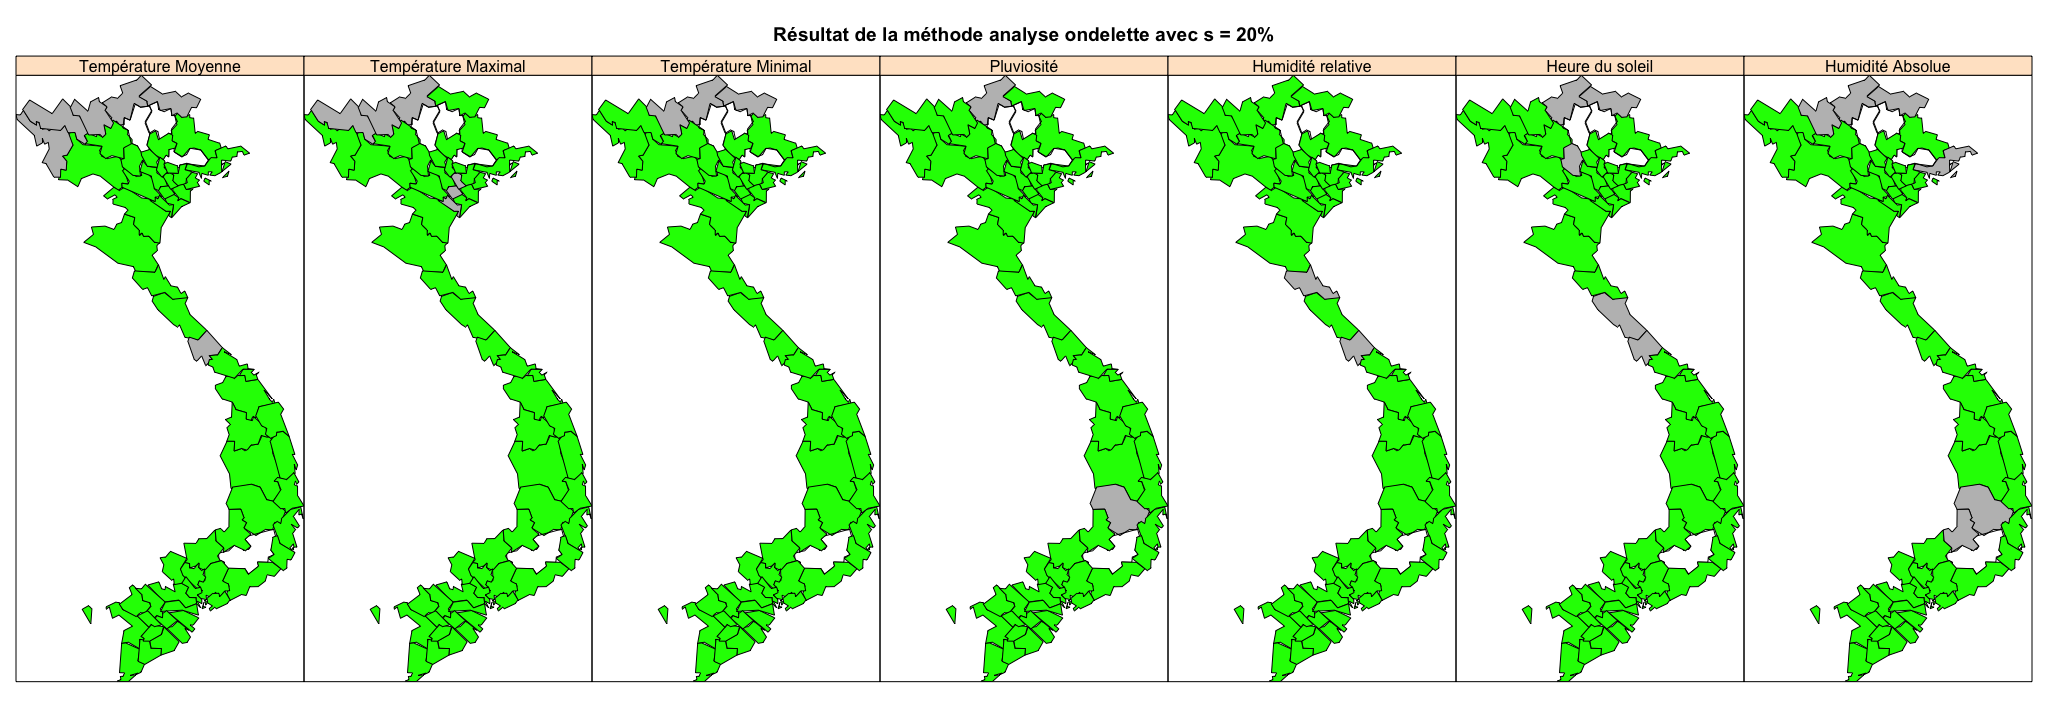
\includegraphics[width = \linewidth]{../figures/chap4/Pic4_6.png}
\caption{Resultat de la méthode d'analyse ondelette sur 64 provinces du Vietnam avec s = 20\%}
\label{Pic4_6}	
\end{figure}

\begin{figure}[h]
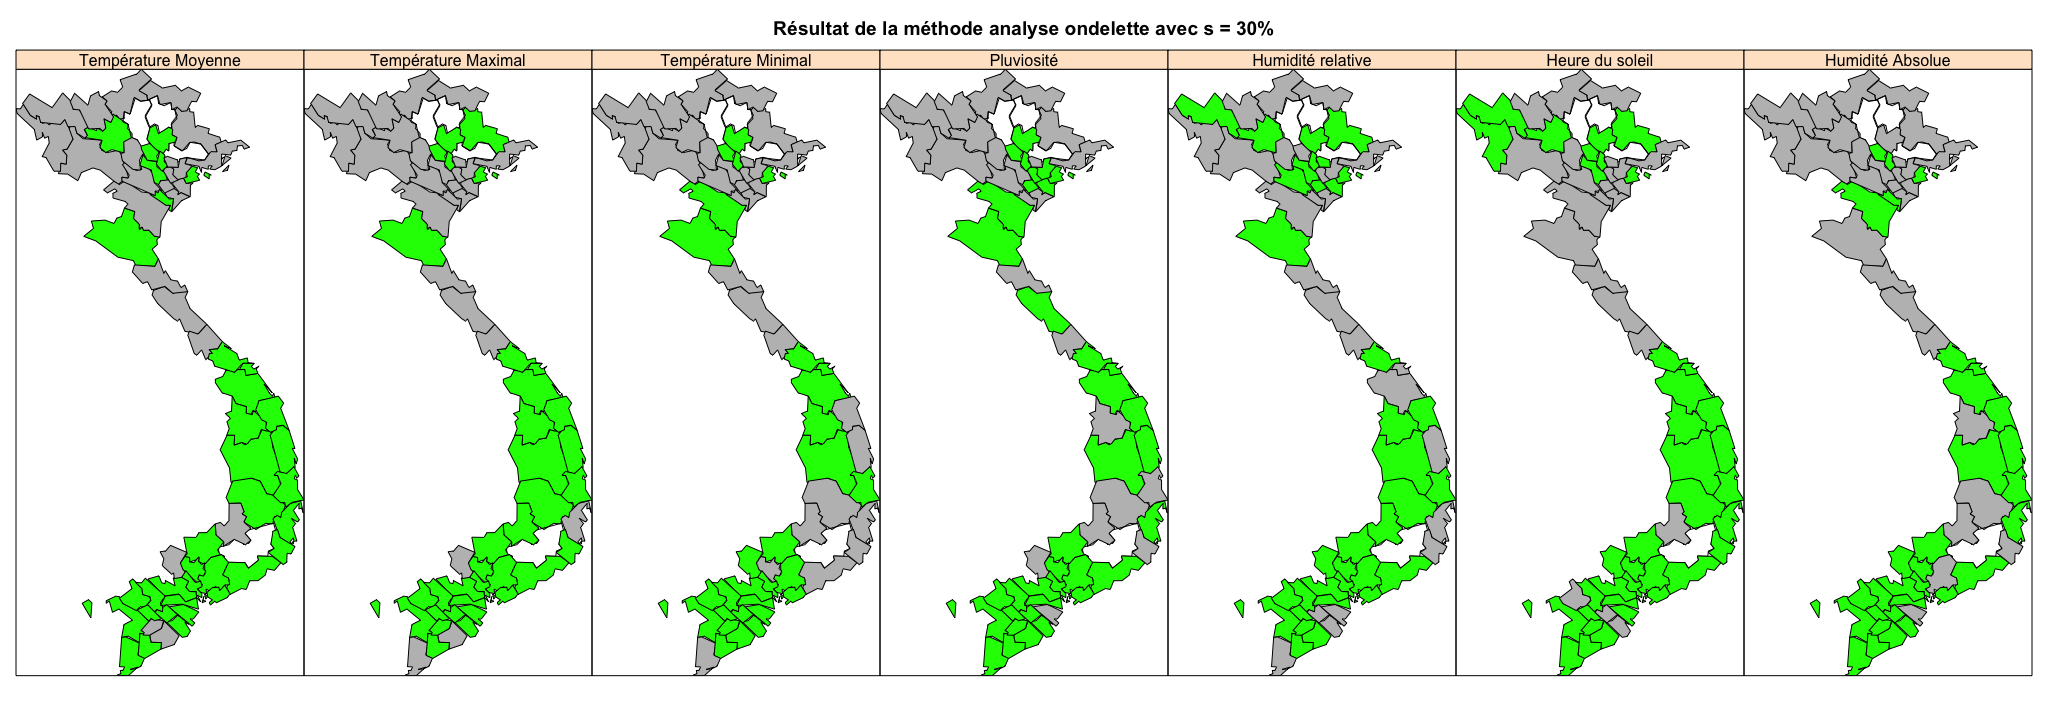
\includegraphics[width = \linewidth]{../figures/chap4/Pic4_7.png}
\caption{Resultat de la méthode d'analyse ondelette sur 64 provinces du Vietnam avec s = 30\%}
\label{Pic4_7}	
\end{figure}

\begin{figure}[h]
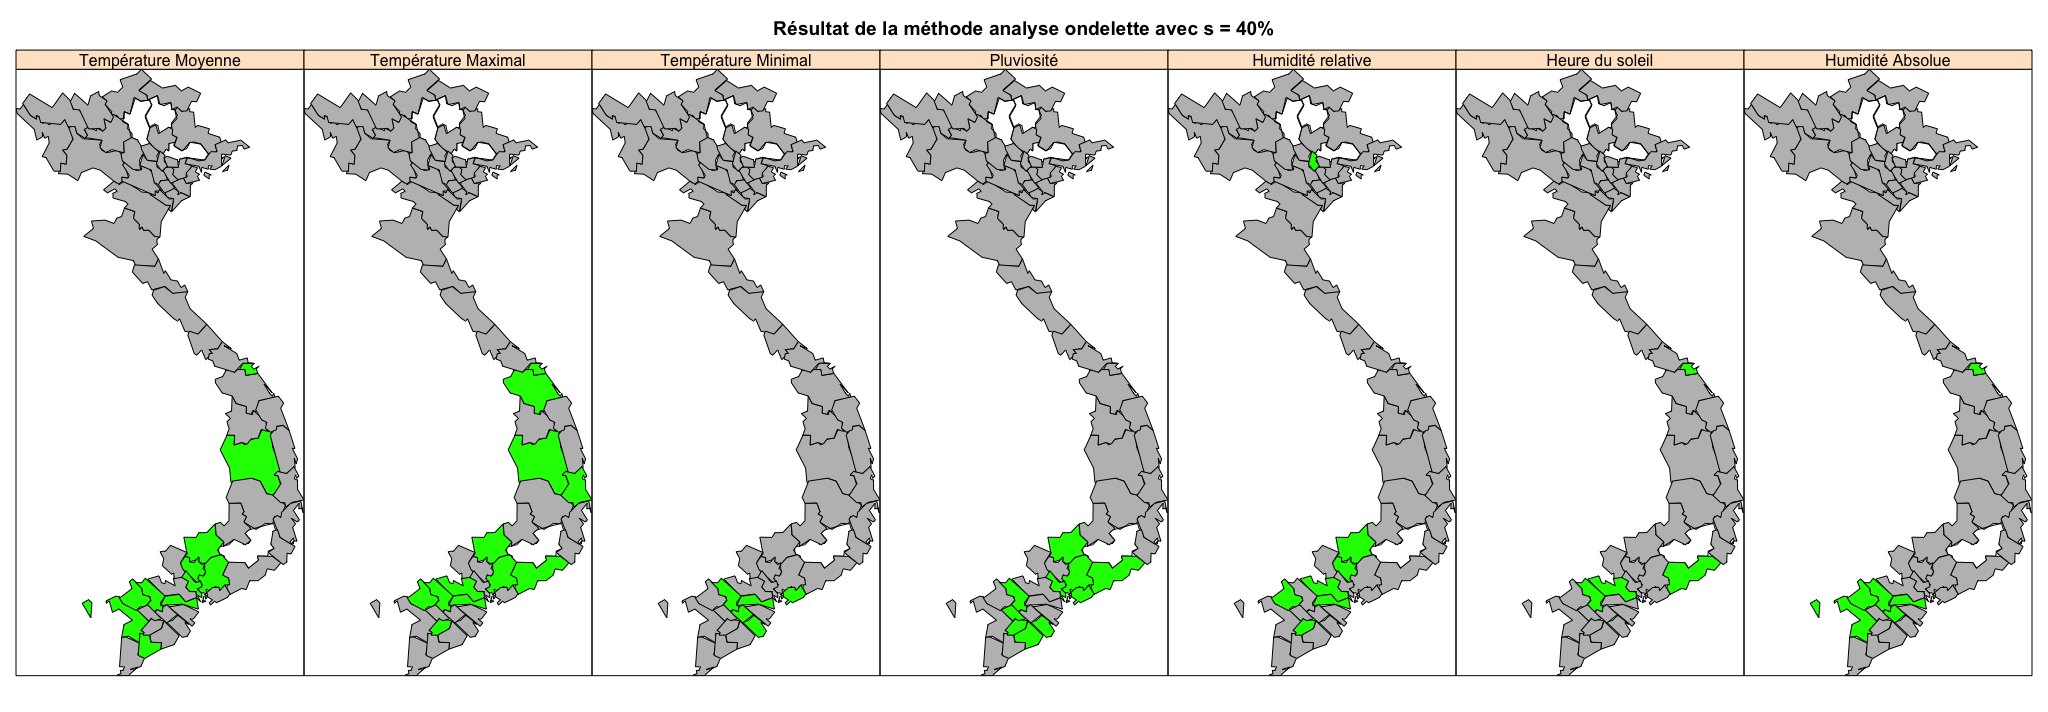
\includegraphics[width = \linewidth]{../figures/chap4/Pic4_8.png}
\caption{Resultat de la méthode d'analyse ondelette sur 64 provinces du Vietnam avec s = 40\%}
\label{Pic4_8}	
\end{figure}

\begin{figure}[h]
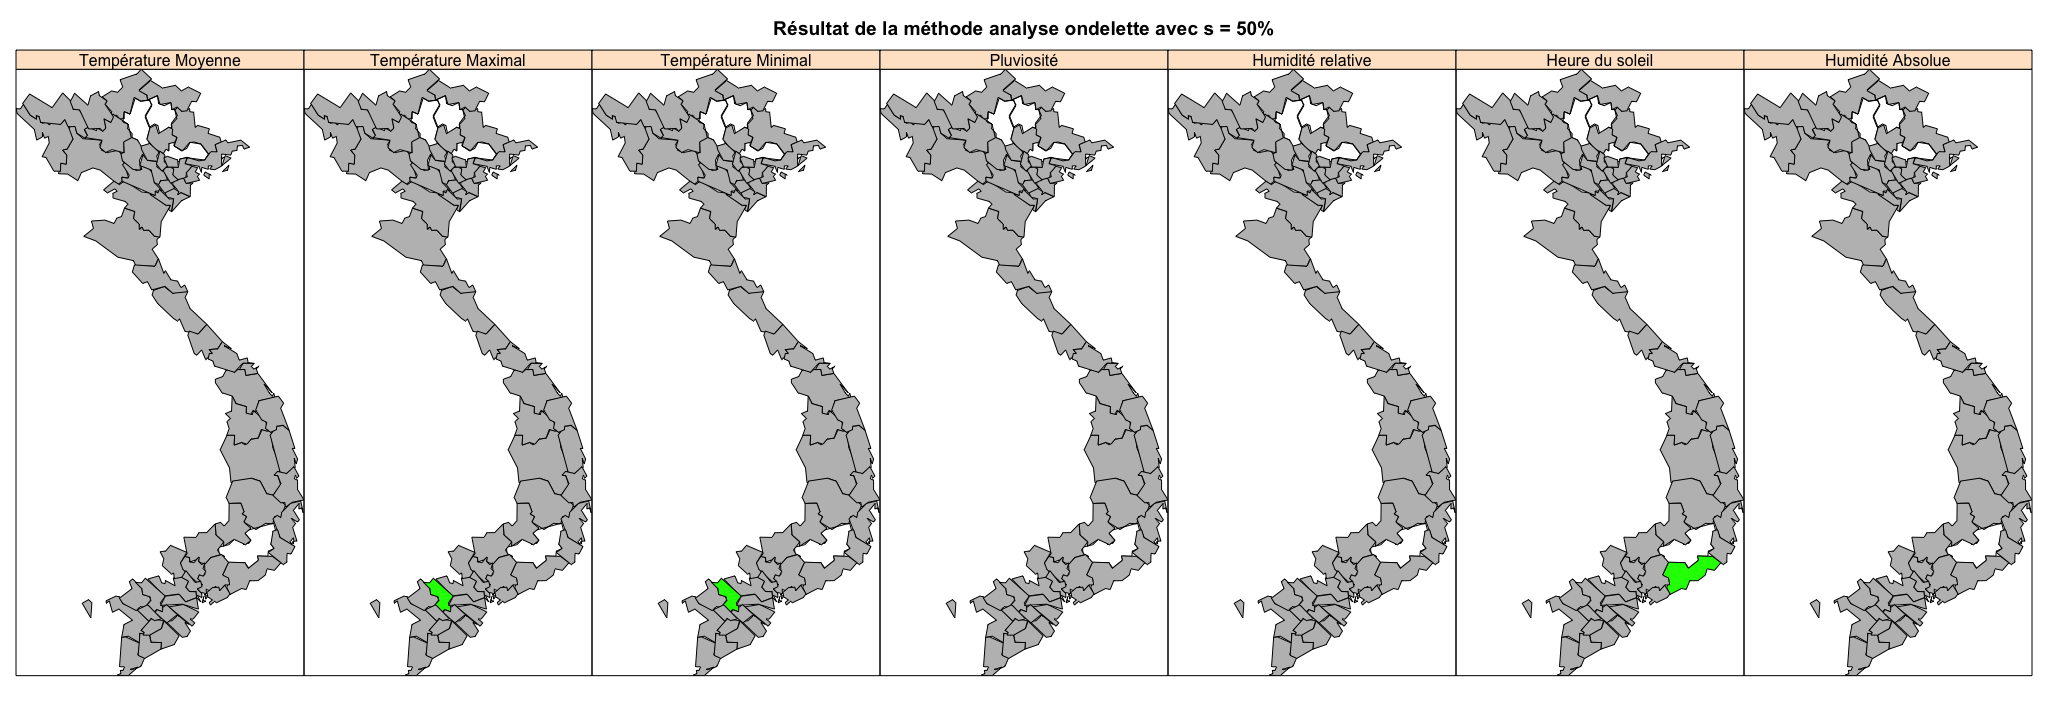
\includegraphics[width = \linewidth]{../figures/chap4/Pic4_9.png}
\caption{Resultat de la méthode d'analyse ondelette sur 64 provinces du Vietnam avec s = 50\%}
\label{Pic4_9}	
\end{figure}


